\section{Non-equilibrium Dynamics}
Today we will discuss the Fokker-Planck equation and how to derive Field theories. We won't have time to discuss anomalous diffusion; how to start with a differential equation that looks like it should scale in an obvious way and then get interesting critical exponents. There's also interesting discussion of analyzing a laser through a statistical field theory lens, which we will not quite get to.

\subsection{Diffusion Equation ($V = 0$)}
Our basic starting point is an equation of motion of the form:
\begin{equation}
    m\ddot{x} = -\frac{\dot{x}}{\mu} - \dpd{V}{x} + f_{\text{noise}}(t)
\end{equation}
i.e. a particle moving deterministically in a potential under the influence of drag and stochastic noise. The potential term leads to ballistic motion, while the noise term leads to diffusive motion. We consider the limit of small $\ddot{x}$ where we can neglect the acceleration term, thus:
\begin{equation}
    \dot{x} = v(x) + \eta(t)
\end{equation}
with:
\begin{equation}
    v(x) = -\mu\dpd{V}{x}
\end{equation}
and:
\begin{equation}
    \avg{\eta} = 0
\end{equation}
\begin{equation}
    \avg{\eta(t)\eta(t')} = 2D\delta(t-t')
\end{equation}
i.e. Markovian white noise.

In the $V = 0$ case, we have the solution:
\begin{equation}
    x(t) = x(0) + \int_0^t dt'\eta(t')
\end{equation}
where:
\begin{equation}
    \avg{(x(t) - x(0))^2} = \int_0^t d\tau_1 \int_0^t d\tau_2 \avg{\eta(\tau_1)\eta(\tau_2)} = 2Dt.
\end{equation}
We then obtain the propagator of the diffusion equation:
\begin{equation}
    P(x, t) = G(x, t, 0, 0) = \frac{1}{(4\pi D t)^{3/2}}e^{-\frac{x^2}{4D}t}
\end{equation}
With $P$ the solution of:
\begin{equation}
    \dpd{P}{t} = -D\nabla^2 P
\end{equation}
this is the familiar diffusion equation.

\subsection{Fokker-Planck Equation ($V \neq 0$)}

Let's now look at advancing time by some small time $\e$:
\begin{equation}
    P(x, t + \e) = \int d^3x' P(x', t)\bra{x}T_\e\ket{x'}
\end{equation}
where $\bra{x}T_\e\ket{x'}$ represents a transition amplitude.

Splitting up the two parts of the motion:
\begin{equation}
    x = x' + v(x)\e + \eta_\e
\end{equation}
where:
\begin{equation}
    \eta_\e = \int_t^{t+\e}dt\eta(t)
\end{equation}
which has the properties:
\begin{equation}
    \avg{\eta_\e} = 0
\end{equation}
\begin{equation}
    \avg{\eta_\e^2} = 6D\e.
\end{equation}
With this, we can define the transition matrix amplitude:
\begin{equation}
    \bra{x}T_\e\ket{x'} = \frac{1}{(4\pi D\e)^{3/2}} \exp(\frac{-(x - x' - \e v(x'))^2}{4D\e})
\end{equation}
Let us explain this. If we had a potential, the particle would have rolled to a specific place deterministically from $x'$. If the particle instead reaches $x$, we need the noise to be precisely the correct magnitude for the particle to get to the position we want it to be, which gives us the above expression. Then:
\begin{equation}
    P(x, t) = \int d^3x' \frac{1}{(4\pi D\e)^{3/2}}P(x', t) \exp(\frac{-(x - x' - \e v(x'))^2}{4D\e})
\end{equation}
for $\abs{x - x'}$ small we can then replace $P(x', t)$ in the integral with $P(x, t)$, and linearize:
\begin{equation}
    \dpd{P}{t} + \nabla \cdot \v{J} = 0 \implies \v{J} = \v{v}P - D\nabla P
\end{equation}
The interpretation of this is intuitive. We have a drift current (from the potential) and a diffusion current (from the noise).

The stationary/equilibrium station is:
\begin{equation}
    P_{\text{eq}}(x) = e^{-V(x)/k_B T}
\end{equation}
with:
\begin{equation}
    \nabla P_{\text{eq}} = \frac{\v{v}}{\mu k_B T}P_{\text{eq}} \implies D = \mu k_B T
\end{equation}
So we identify what the parameter $D$ must be. This is usually called the ``fluctuation-dissipation'' theorem.

\subsection{Generalizing to a field - Model A}
We write down the Hamiltonian as a function of a field $m$:
\begin{equation}
    H[m] = \int d^dx \left(\frac{1}{2}rm^2 + \frac{1}{4}um^4 + \frac{1}{2}\kappa (\nabla m)^2 + \ldots \right)
\end{equation}
The analogous EoM is:
\begin{equation}
    \dpd{m}{t} = -\mu\frac{\delta H}{\delta m} + \eta(t) = -\mu r m - \mu u m^3 + \mu \kappa(\nabla^2 m) + \eta
\end{equation}

In the Gaussian theory (taking $u = 0$) we have:
\begin{equation}
    \dpd{m(q, t)}{t} = -\mu(r + \kappa q^2)m + \eta
\end{equation}
where:
\begin{equation}
    \avg{\eta} = 0
\end{equation}
\begin{equation}
    \avg{\eta_q\eta_{q'}} = 2D\delta(t-t')\delta(q-q')(2\pi)^d
\end{equation}
There is then a $q$-mode decay time:
\begin{equation}
    \frac{1}{\tau(q)} = \mu(r + \kappa q^2)
\end{equation}
from this we can determine what happens to the fluctuations:
\begin{equation}
    \avg{m(q, t)m(q', t)} = \frac{D\delta(q + q')}{\mu(v + \kappa q^2)}
\end{equation}
where there is no time-dependence for we have performed an ensemble average. At very long times the distribution approaches the Lorentzian. Note that $\frac{D}{\mu} = k_B T$. This is what is known as ``critical slowing down''.

In some sense we pulled the EoM out of a hat, and its not the most general EoM we could have written down. In particular we notice the order parameter is not conserved. This specific model is known as model A. There are models A-F, check out the review article by Honenberg in reviews of modern physics if interested. But for now, we only study A/B.

\subsection{Model B}
Now consider a model where we do want the order parameter to be conserved:
\begin{equation}
    \dod{}{t}\int d^dx m(x, t) = 0
\end{equation}
so we now have the equation of motion:
\begin{equation}
    \dpd{m}{t} = -\nabla j + \nabla \sigma
\end{equation}
with $j = \mu v$ and $\sigma \sim \eta$. This new model has the constraint that the magnetization is fixed, and this gets rid of low-order derivatives. We thus end up with:
\begin{equation}
    \dpd{m}{t} = \mu v \nabla^2 m - \mu \kappa \nabla^4 m + \eta
\end{equation}
Thus we have different dynamics associated with the conservation of the order parameter.

\subsection{Noise and Optimal Trajectories}
The above was all pretty heuristic. Let's explore something that's less heuristic, with a similar starting point:
\begin{equation}
    \dot{X} = A(X) + B\xi
\end{equation}
with $\avg{\xi\xi} = 2D\delta(t - t')$. 

We solve this via the identity:
\begin{equation}
    1 = Z[\xi] = \int \mathcal{D}X(t)\;J(X)\delta[\p_t X - A(X) - B\xi]
\end{equation}
where we have stuck in the EoM as a delta function.

We then generate an auxilary field $X^q$ using an identity:
\begin{equation}
    Z[\xi] = \int \mathcal{D}X(t)\int \mathcal{D}X^q(t)\exp(-2i\int dt X^q(t)(\p_t X - A - B\xi))
\end{equation}
Why we set this up is so that we can integrate over the noise (also let's set $B = 1$):
\begin{equation}
    Z = \int \mathcal{D}\xi e^{-\frac{1}{4}\int dt \xi^2}Z[\xi] = \int \mathcal{D}X\mathcal{D}X^q \exp(\int dt \left[-2iX^q(\p_t X - A(X)) - 4(X^q)^2\right])
\end{equation}
We now have an action that is a function of two fields. Faced with something like this, we look at the saddle point equations (here of two variables). This yields two equations:
\begin{equation}
    \dot{X} = A(X) + 4iX^qD(X)
\end{equation}
\begin{equation}
    i\dot{X}^q = -iX^qA'(X) + 2(X^q)^2D'
\end{equation}
with $' = \dpd{}{X}$. $X^q$ must be imaginary since $X$ is real. Let us do a change of variables $P = 2iX^q$. In this case, it turns out that we can write the equations of motion we saw above as:
\begin{equation}
    \dot{X} = \p_P H[P, X]
\end{equation}
\begin{equation}
    \dot{P} = -\p_X H[P, X]
\end{equation}
with:
\begin{equation}
    H = PA(X) + P^2 D(X).
\end{equation}
These look exactly like Hamilton's equations! $X^q$ ``looks like'' a conjugate momentum. We can then identify an action:
\begin{equation}
    iS[X, P] = - \int dt [P\dot{X} - H]
\end{equation}
and think about optimal trajectories. The simplest one to think about would be to take $A(X) = -\dpd{V}{X}$, Since $D(X) \sim T$, we have two stable trajectories where $H$ is zero; when $P = 0$, or when $P = -\frac{A}{D}$. Sketching the flows in phase space:

\begin{center}
    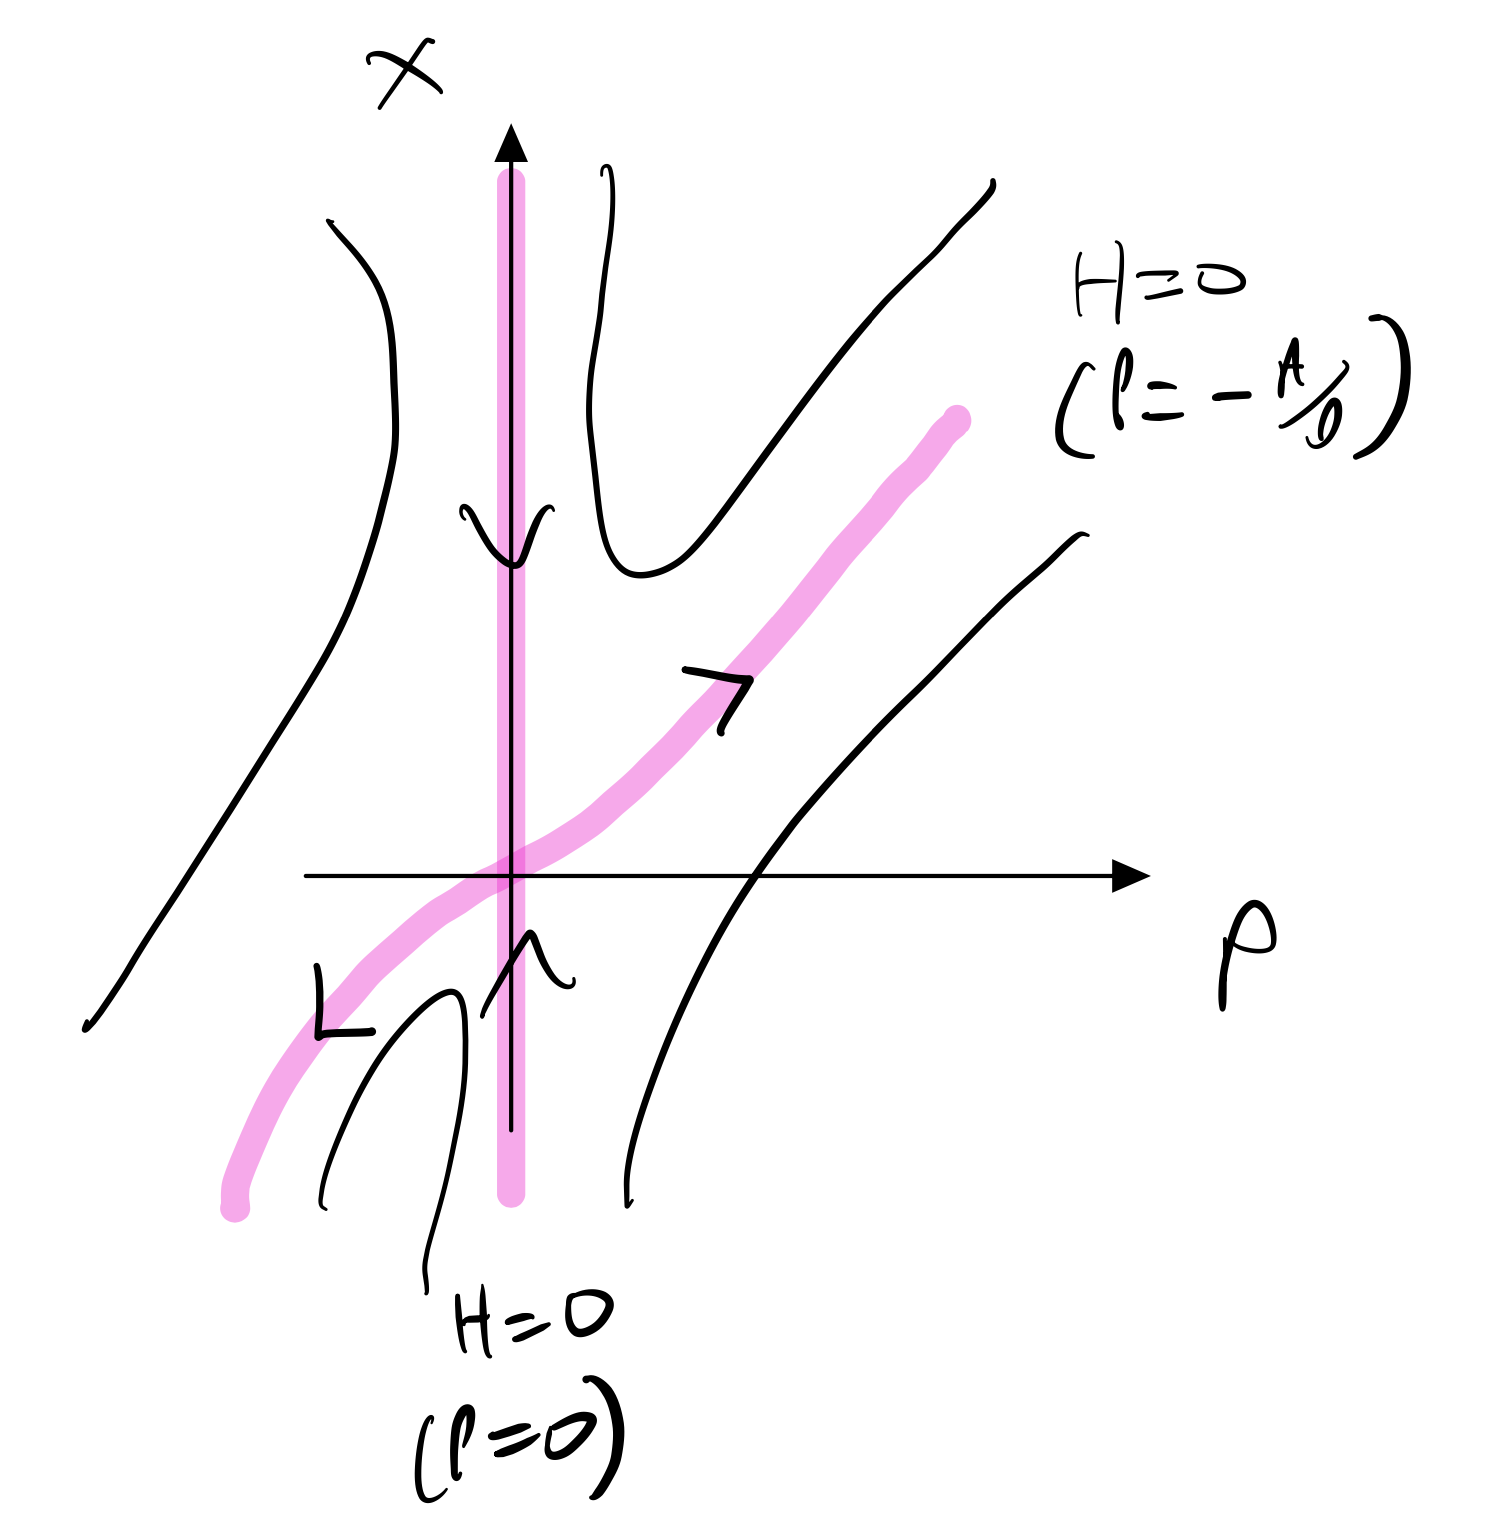
\includegraphics[scale=0.3]{Lectures/Figures/lec16-phasespace.png}
\end{center}

In equilibrium of this problem, what is $P(X_0)$? Let us write the action:
\begin{equation}
    iS[X_0] = - \int dt P\dot{X} = -\int_0^{X_0}P(X)
\end{equation}
Then taking $P(X) = -\frac{A}{D} = -\frac{V'}{D}$:
\begin{equation}
    iS[X_0] = -\frac{1}{T}\int_0^{X_0}dx V'(X) = \frac{1}{T}(V - V_0)
\end{equation}
which is just the Boltzmann distribution!

A last point. Suppose the potential has a metastable minimum:

\begin{center}
    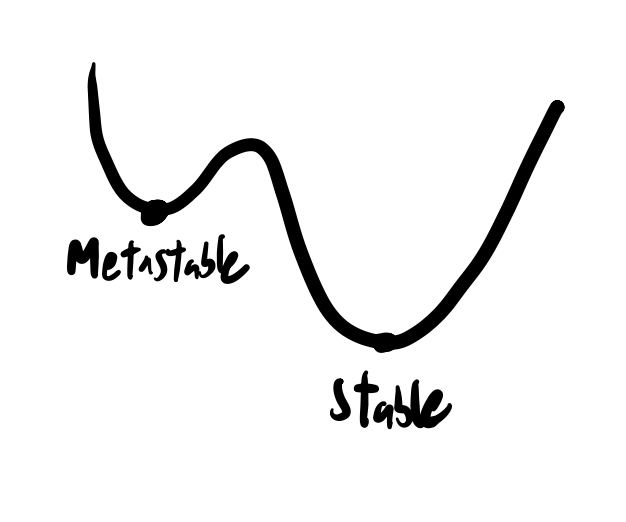
\includegraphics[scale=0.4]{Lectures/Figures/lec16-metastableminima.png}
\end{center}

Then, what I am interested in is the probability of escape, given by the shaded region:

\begin{center}
    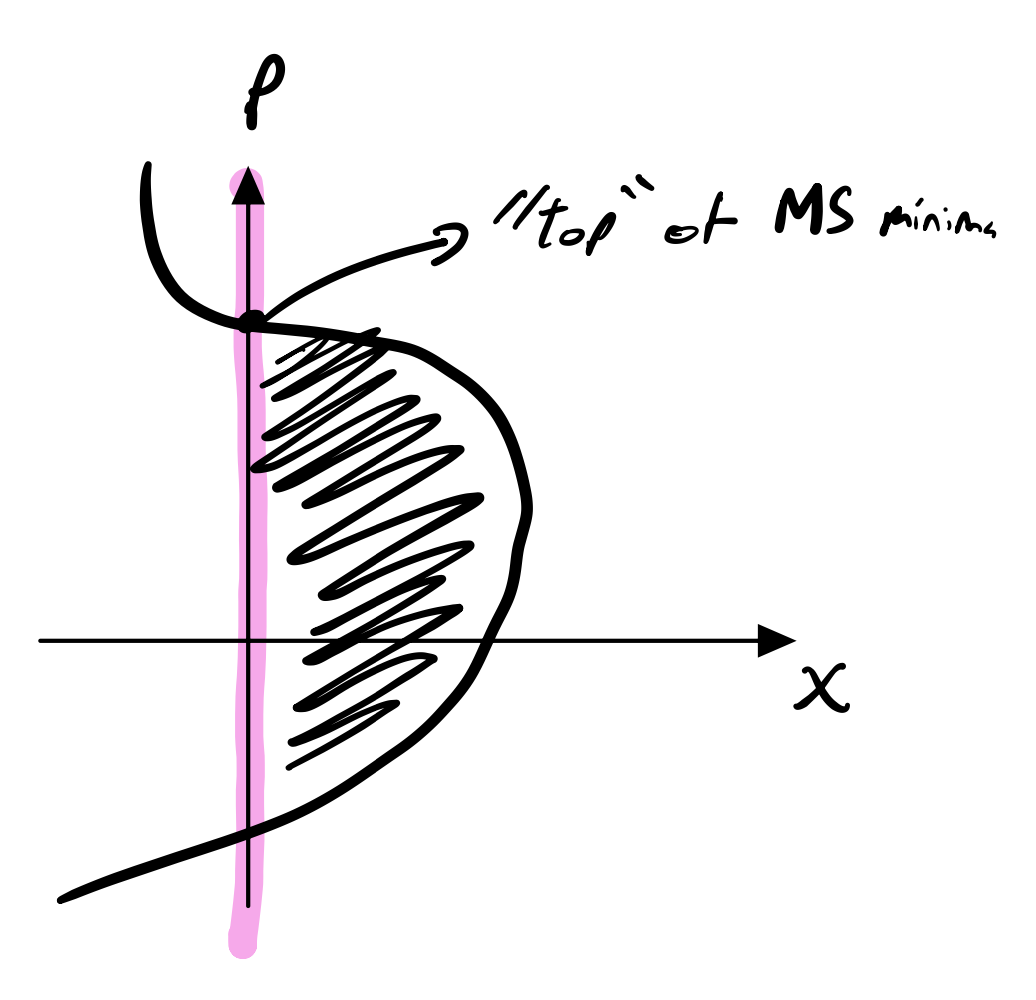
\includegraphics[scale=0.3]{Lectures/Figures/lec16-metastablephase.png}
\end{center}

which gives:
\begin{equation}
    S[X_S] = -\frac{V(X_S) - V(0)}{T}
\end{equation}
which is just WKB.

Here, we find an optimal trajectory, which gives us where we want to be. This is of course an approximation. We can go back and add more terms to our theory, making it a dynamical field theory. 

Note: The best review of this material comes from Kamenev.

\subsection{Where have we come?}
There are generic and universal properties of theories. They are made most evident at the point where these theories are hardest to solve. The underlying principle behind this universality is scaling and embodied by the renormalization group. The definition of the interesting point/phase transition is associated with the scale invariant quantities. This doesn't always happen, and almost any real system deviates from this, but such deviation can itself lead to interesting phenomenology, e.g. in the case of disorder and spin glasses.

If you have the time, next week we'll discuss quantum critical points (adding back the non-linear terms and seeing their effects). We will also study the laser and fluids/porous media, which gives us anomalous scaling/stretched power laws. 